\documentclass[12pt]{scrartcl}

\usepackage[
  a4paper, mag=1000,
  left=2cm, right=1cm, top=2cm, bottom=2cm, headsep=0.7cm, footskip=1.27cm
]{geometry}

\usepackage[T2A]{fontenc}
\usepackage[utf8]{inputenc}
\usepackage[english,russian]{babel}
\usepackage{cmap}
\usepackage{amsmath}
\usepackage{tabularx}
\usepackage{graphicx}
\usepackage{array}
\IfFileExists{pscyr.sty}{\usepackage{pscyr}}{}
\usepackage[parfill]{parskip}
\usepackage{lastpage}
\usepackage{setspace} % single spacing between lines
\usepackage{blindtext} % for generated text - can remove
\usepackage{titlesec} % set header spacing
\setlength{\parindent}{15pt} % paragraph indent

\titlespacing{\section}{0pt}{\parskip}{-\parskip}
\titlespacing{\subsection}{0pt}{\parskip}{-\parskip}
\titlespacing{\subsubsection}{0pt}{\parskip}{-\parskip}

\usepackage[numbered]{bookmark}
\clubpenalty=10000
\widowpenalty=10000

\usepackage{fancybox,fancyhdr}
\pagestyle{fancy}
\fancyhf{}
\fancyhead[C]{\small{Олимпиадное программирование (средний уровень). Тренировка 02 \\ Летняя компьютерная школа ``КЭШ'', 6--26 августа 2016 года}}

%user-defined commands

\newcommand{\inputFile}{Стандартный ввод}
\newcommand{\outputFile}{Стандартный вывод}

\begin{document}

\singlespacing

\section*{Задача A. Простое число}

\begin{tabularx}{\textwidth}{l l X}
    Имя входного файла: & \texttt{\inputFile} \\
    Имя выходного файла: & \texttt{\outputFile} \\
    Ограничение по времени: & $2$ секунды \\
    Ограничение по памяти: & $256$ мегабайт \\
\end{tabularx}

\begin{figure}[h]
    
\includegraphics[scale=0.5]{jake}
\end{figure}

В Землях ООО живет обычный паренек Финн и его друг~---~волшебный пес Джейк. 
Они живут в доме на дереве в Конфетном королевстве. Джейк умеет растягиваться и управлять формой своего тела, превращаясь во что угодно. Однако,после сражения с одним очень опасным монстром, он не может растягиваться на количество метров, которое является \emph{простым числом}. Простое число~---~это такое число, которое делится только на себя и на 1. Помогите Джейку найти такие числа!

\subsection*{Формат входных данных}
На вход Джейк подает одно число~---~то число, на которое он хочет растянуться.


\subsection*{Формат выходных данных}
Вы должны вевести \emph{``YES''}, если число является простым, в противном случае~---~\emph{``NO''}


\subsection*{Примеры}

\texttt
{
	\begin{tabularx}{0.9\textwidth}{| X | X |}
       \hline
       \multicolumn{1}{|c|}{\inputFile} & \multicolumn{1}{c|}{\outputFile} \\ 
       \hline 
       4 & NO \\
       \hline
       7 & YES \\
       \hline
    \end{tabularx}
}

\newpage

\section*{Задача B. Пингвинские треугольники}

\begin{tabularx}{\textwidth}{l l X}
    Имя входного файла: & \texttt{\inputFile} \\
    Имя выходного файла: & \texttt{\outputFile} \\
    Ограничение по времени: & $2$ секунды \\
    Ограничение по памяти: & $256$ мегабайт \\
\end{tabularx}

\begin{figure}[h]
    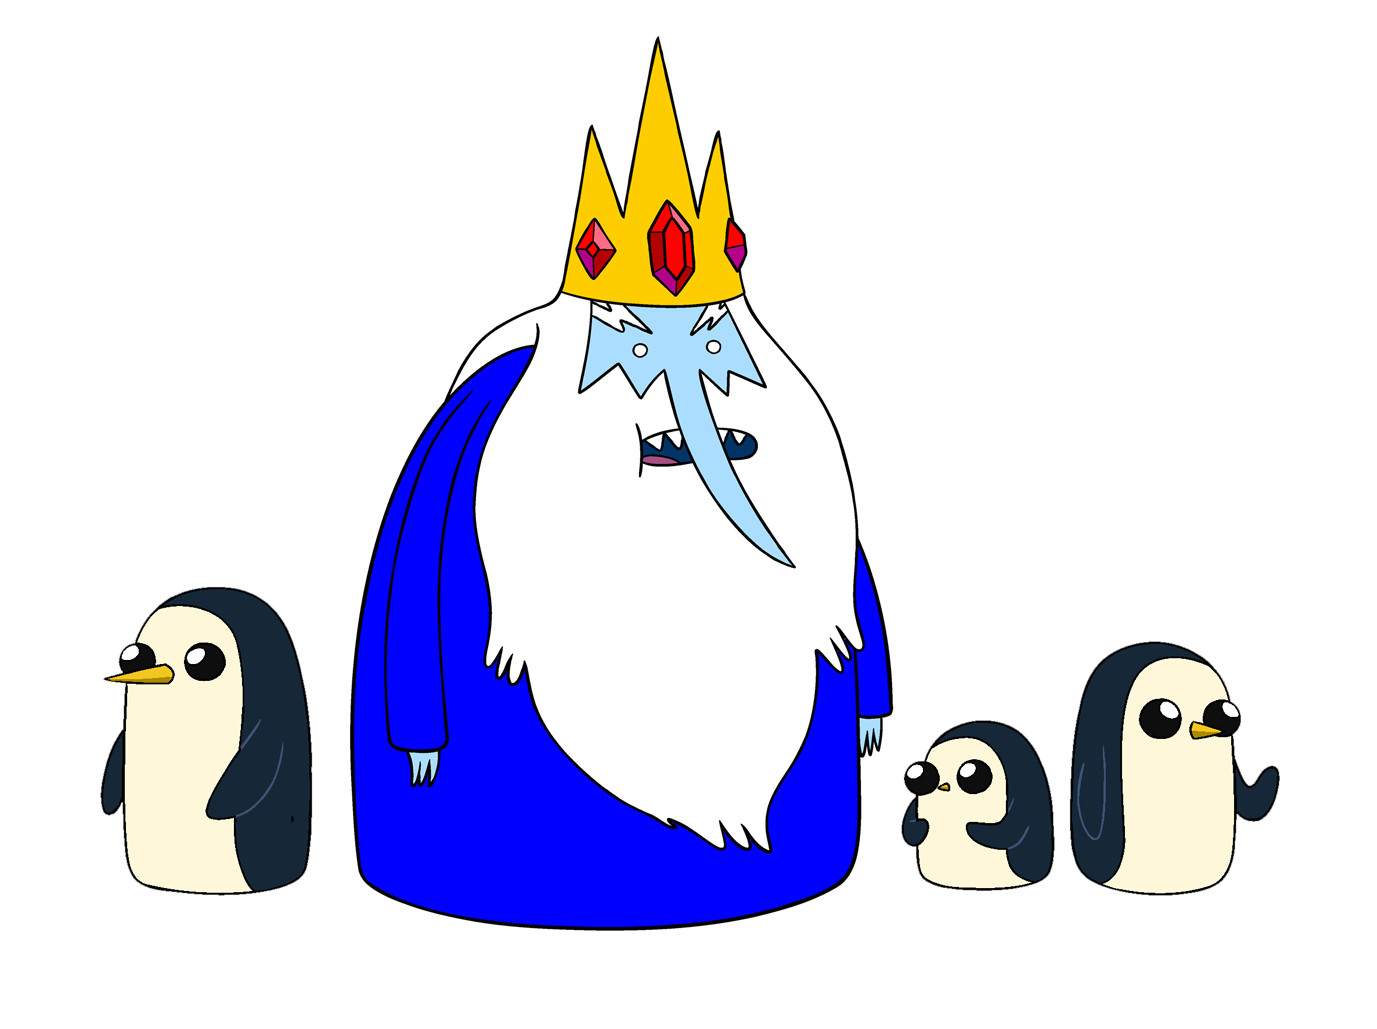
\includegraphics[scale=0.6]{iceKing}
\end{figure}

Знакомьтесь~---~это Ледяной Король и его подручные пингвины. Они живут в Ледяном Королестве на большой-большой горе. Ледяной Король хочет жениться на какой-нибудь принцессе, однако пока ни одна из них не осталась с ним надолго, так как все считают его достаточно скучным и странным. Для развлечения возможных будущих невест король решил построить ледяную горку из пингвинов~---~они должны построиться в треугольник со сторонами \emph{a}, \emph{b}, \emph{c}, а затем они будут на время заморожены Королем. Однако он прочитал в своей библиотеке, что самые лучшие и захватывающие ледяные горки (они же пингвинские) получаются в том случае, если стороны горки-треугольника будут подчинены следующему выражению: $a^2 + b^2 = c^2$ и $a < b < c$. Так же у него в наличии мало пингвинов, из которых можно сделать горку, поэтому стороны ограничены числом $N$. Помоги ему найти всевозможные варианты пингвинских горок, которые можно построить.

\subsection*{Формат входных данных}
На вход подается $N$~---~максимальное количество пингвинов, которое можно задействовать в стороне горки-треугольника.

\subsection*{Формат выходных данных}
Вывести значения $a$, $b$ и $c$, удолетворяющих условию, через пробел. Если таких несколько, то вывести все, используя перевод строки.

\subsection*{Примеры}

\texttt
{
	\begin{tabularx}{0.9\textwidth}{| X | X |}
       \hline
       \multicolumn{1}{|c|}{\inputFile} & \multicolumn{1}{c|}{\outputFile} \\ 
       \hline 
       10 &
       \parbox[t]{\textheight}
       {
         3 4 5  \\
         6 8 10 \\      
       } \\
       \hline
    \end{tabularx}
}

\newpage

\section*{Задача C. Счастливые билетики}

\begin{tabularx}{\textwidth}{l l X}
    Имя входного файла: & \texttt{\inputFile} \\
    Имя выходного файла: & \texttt{\outputFile} \\
    Ограничение по времени: & $2$ секунды \\
    Ограничение по памяти: & $256$ мегабайт \\
\end{tabularx}

\begin{figure}[h]
    
\includegraphics[scale=0.6]{lsp}
\end{figure}

Принцессу Пупырчатого Королевства (Принцессу Пупырку) выгнали из дома свои собственные родители из-за постоянных ссор ввиду скверного характера. Теперь она живет где-то в Конфетном Королестве и ей очень не хватает денег! Но работать она не желает~---~принцессы ведь не работают! Поэтому она занимает денег у своих подруг и тратит их на лотерейные билетики. Каждый билетик состоит из 6 цифр. Он является \emph{счастливым}, т.е. выигрышным, если сумма первых трех чисел равна сумме последних трех чисел. Помогите Принцессе Пупырке найти всевозможные счастливые билетики.

\subsection*{Формат входных данных}
Отсуствует~---~т.е. на вход ничего не подается.

\subsection*{Формат выходных данных}
Вывести все возможные варианты счастливых билетиков: каждый вариант на отдельной строке.

\end{document}
